\chapter{About the Author}
Robert Burton was the son of Ralph Burton, of an ancient and genteel family at Lindley, in Leicestershire, and was born there on the 8th of February 1576.
He received the first rudiments of learning at the free school of Sutton Coldfield, in Warwickshire\footnoteA{This is Wood's account.
His will says, Nuneaton; but a passage in this work (see \autopageref{mention:coldfield}) mentions Sutton Coldfield; probably he may have been at both schools.} from whence he was, at the age of seventeen, in the long vacation, 1593, sent to Brazen Nose College, in the condition of a commoner, where he made considerable progress in logic and philosophy.
In 1599 he was elected student of Christ Church, and, for form's sake, was put under the tuition of Dr. John Bancroft, afterwards Bishop of Oxford.
In 1614 he was admitted to the reading of the Sentences, and on the 29th of November, 1616, had the vicarage of St. Thomas, in the west suburb of Oxford, conferred on him by the dean and canons of Christ Church, which, with the rectory of Segrave, in Leicestershire, given to him in the year 1636, by George, Lord Berkeley, he kept, to use the words of the Oxford antiquary, with much ado to his dying day.
He seems to have been first beneficed at Walsby, in Lincolnshire, through the munificence of his noble patroness, Frances, Countess Dowager of Exeter, but resigned the same, as he tells us, for some special reasons.
At his vicarage he is remarked to have always given the sacrament in wafers.
Wood's character of him is, that \blockquote{he was an exact mathematician, a curious calculator of nativities, a general read scholar, a thorough-paced philologist, and one that understood the surveying of lands well.
As he was by many accounted a severe student, a devourer of authors, a melancholy and humorous person; so by others, who knew him well, a person of great honesty, plain dealing and charity.
I have heard some of the ancients of Christ Church often say, that his company was very merry, facete, and juvenile; and no man in his time did surpass him for his ready and dexterous interlarding his common discourses among them with verses from the poets, or sentences from classic authors; which being then all the fashion in the University, made his company the more acceptable.}

He appears to have been a universal reader of all kinds of books, and availed himself of his multifarious studies in a very extraordinary manner.
From the information of Hearne, we learn that John Rouse, the Bodleian librarian, furnished him with choice books for the prosecution of his work.
The subject of his labour and amusement, seems to have been adopted from the infirmities of his own habit and constitution.
Mr. Granger says, \blockquote{He composed this book with a view of relieving his own melancholy, but increased it to such a degree, that nothing could make him laugh, but going to the bridge-foot and hearing the ribaldry of the bargemen, which rarely failed to throw him into a violent fit of laughter.
Before he was overcome with this horrid disorder, he, in the intervals of his vapours, was esteemed one of the most facetious companions in the University}.

His residence was chiefly at Oxford; where, in his chamber in Christ Church College, he departed this life, at or very near the time which he had some years before foretold, from the calculation of his own nativity, and which, says Wood,
\enquote{being exact, several of the students did not forbear to whisper among themselves, that rather than there should be a mistake in the calculation, he sent up his soul to heaven through a slip about his neck.}. Whether this suggestion is founded in truth, we have no other evidence than an obscure hint in the epitaph hereafter inserted, which was written by the author himself, a short time before his death. His body, with due solemnity, was buried near that of Dr. Robert Weston, in the north aisle which joins next to the choir of the cathedral of Christ Church, on the 27th of January 1639-40.
Over his grave was soon after erected a comely monument, on the upper pillar of the said aisle, with his bust, painted to the life. On the right hand is the following calculation of his nativity:
\\
\\
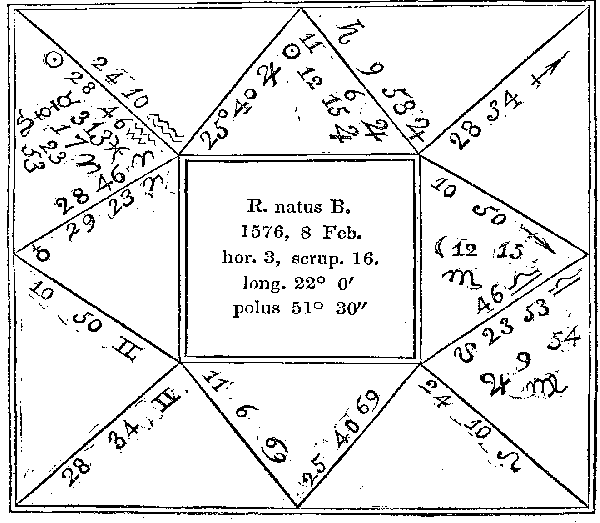
\includegraphics[width=\textwidth,keepaspectratio]{horoscope}

and under the bust, this inscription of his own composition:

\settowidth{\versewidth}{Paucis notus, paucioribus ignotus,}
\begin{verse}[\versewidth]
Paucis notus, paucioribus ignotus,\\*
Hic jacet Democritus junior\\*
Cui vitam dedit et mortem\\*
Melancholia\\*
\hrulefill\\*
Obiit 8 Idus Januarii. A. C. {\junicoderomannumerals{MDCXXXIX}}.\\!
\end{verse}

Freely translated:

\settowidth{\versewidth}{Known to few, unknown to fewer,}
\begin{verse}[\versewidth]
Known to few, unknown to fewer,\\*
Here lies Democritus Junior,\\*
to whom Melancholy gave\\*
both life and death\\!
\end{verse}

%Arms:—Azure on a bend O. between three dogs' heads O. a crescent G.

A few months before his death, he made his will, of which the following is a copy:
\\

{\scriptsize{}\lq\lq\textbf{EXTRACTED FROM THE REGISTRY OF THE PREROGATIVE COURT OF CANTERBURY.}

\emph{In nomine Dei Amen.} August 15th One thousand six hundred thirty nine because there be so many casualties to which our life is subject besides quarrelling and contention which happen to our Successors after our Death by reason of unsettled Estates I Robert Burton Student of Christ-church Oxon. though my means be but small have thought good by this my last Will and Testament to dispose of that little which I have and being at this present I thank God in perfect health of Bodie and Mind and if this Testament be not so formal according to the nice and strict terms of Law and other Circumstances peradventure required of which I am ignorant I desire howsoever this my Will may be accepted and stand good according to my true Intent and meaning.

First I bequeath Animam Deo Corpus Terrae whensoever it shall please God to call me I give my Land in Higham which my good Father Ralphe Burton of Lindly in the County of Leicester Esquire gave me by Deed of Gift and that which I have annexed to that Farm by purchase since, now leased for thirty eight pounds per Ann. to mine Elder Brother William Burton of Lindly Esquire during his life and after him to his Heirs I make my said Brother William likewise mine Executor as well as paying such Annuities and Legacies out of my Lands and Goods as are hereafter specified I give to my nephew Cassibilan Burton twenty pounds Annuity per Ann. out of my Land in Higham during his life to be paid at two equal payments at our Lady Day in Lent and Michaelmas or if he be not paid within fourteen Days after the said Feasts to distrain on any part of the Ground or on any of my Lands of Inheritance Item I give to my Sister Katherine Jackson during her life eight pounds per Ann. Annuity to be paid at the two Feasts equally as above said or else to distrain on the Ground if she be not paid after fourteen days at Lindly as the other some is out of the said Land Item I give to my Servant John Upton the Annuity of Forty Shillings out of my said Farme during his life (if till then my Servant) to be paid on Michaelmas day in Lindley each year or else after fourteen days to distrain Now for my goods I thus dispose them First I give an C'th pounds to Christ Church in Oxford where I have so long lived to buy five pounds Lands per Ann. to be Yearly bestowed on Books for the Library Item I give an hundredth pound to the University Library of Oxford to be bestowed to purchase five pound Land per Ann. to be paid out Yearly on Books as Mrs. Brooks formerly gave an hundred pounds to buy Land to the same purpose and the Rent to the same use I give to my Brother George Burton twenty pounds and my watch I give to my Brother Ralph Burton five pounds Item I give to the Parish of Seagrave in Leicestershire where I am now Rector ten pounds to be given to a certain Feoffees to the perpetual good of the said Parish Oxon Item I give to my Niece Eugenia Burton One hundredth pounds Item I give to my Nephew Richard Burton now Prisoner in London an hundredth pound to redeem him Item I give to the Poor of Higham Forty Shillings where my Land is to the poor of Nuneaton where I was once a Grammar Scholar three pound to my Cousin Purfey of Wadlake my Cousin Purfey of Calcott my Cousin Hales of Coventry my Nephew Bradshaw of Orton twenty shillings a piece for a small remembrance to Mr. Whitehall Rector of Cherkby myne own Chamber Fellow twenty shillings I desire my Brother George and my Cosen Purfey of Calcott to be the Overseers of this part of my Will I give moreover five pounds to make a small Monument for my Mother where she is buried in London to my Brother Jackson forty shillings to my Servant John Upton forty shillings besides his former Annuity if he be my Servant till I die if he be till then my Servant

-- ROBERT BURTON

-- Charles Russell, Witness

-- John Pepper, Witness.

An Appendix to this my Will if I die in Oxford or whilst I am of Christ Church and with good Mr. Paynes August the Fifteenth 1639.

I give to Mr. Doctor Fell Dean of Christ Church Forty Shillings to the Eight Canons twenty Shillings a piece as a small remembrance to the poor of St. Thomas Parish Twenty Shillings to Brasenose Library five pounds to Mr. Rowse of Oriell Colledge twenty Shillings to Mr. Heywood xxs. to Dr. Metcalfe xxs. to Mr. Sherley xxs. If I have any Books the University Library hath not, let them take them If I have any Books our own Library hath not, let them take them I give to Mrs. Fell all my English Books of Husbandry one excepted to her Daughter Mrs. Katherine Fell my Six Pieces of Silver Plate and six Silver spoons to Mrs. Iles my Gerards Herball To Mrs. Morris my Country Farme Translated out of French 4. and all my English Physick Books to Mr. Whistler the Recorder of Oxford I give twenty shillings to all my fellow Students Mrs of Arts a Book in fol. or two a piece as Master Morris Treasurer or Mr. Dean shall appoint whom I request to be the Overseer of this Appendix and give him for his pains Atlas Geografer and Ortelius Theatrum Mond' I give to John Fell the Dean's Son Student my Mathematical Instruments except my two Crosse Staves which I give to my Lord of Donnol if he be then of the House To Thomas Iles Doctor Iles his Son Student Saluntch on Paurrhelia and Lucian's Works in 4 Tomes If any books be left let my Executors dispose of them with all such Books as are written with my own hands and half my Melancholy Copy for Crips hath the other half To Mr. Jones Chaplin and Chanter my Surveying Books and Instruments To the Servants of the House Forty Shillings

-- ROBERT BURTON

-- Charles Russell, Witness

-- John Pepper, Witness

--- This Will was shewed to me by the Testator and acknowledged by him some few days before his death to be his last Will Ita Testor John Morris S Th D. Prebendari' Eccl Chri' Oxon Feb. 3, 1639. Probatum fuit Testamentum suprascriptum, \etc. 11° 1640 Juramento Willmi Burton Fris' et Executoris cui \etc{} de bene et fideliter administrand. \etc{} coram Mag'ris Nathanaele Stephens Rectore Eccl. de Drayton, et Edwardo Farmer, Clericis, vigore commissionis, \etc.\rq\rq}
